%%%%%%%%%%%%%%%%%%%%%%%%%%%%%%%%%%%%%%%%%%%%%%%%%%%%%%%%%%%%%%%%
% Tipo de documento y paquetes
\documentclass[10pt]{book}
\usepackage{cdt/cdtAnalisis}
\usepackage{subfigure}
\usepackage{appendix}

%%%%%%%%%%%%%%%%%%%%%%%%%%%%%%%%%%%%%%%%%%%%%%%%%%%%%%%%%%%%%%%%
% Colores
\let\TAB\tabular
\renewcommand\tabular{\noindent\TAB}
\definecolor{gray1}{gray}{0.89}%{0.80}
\definecolor{gray2}{gray}{0.68}
\definecolor{gray3}{gray}{0.97}
\definecolor{pink1}{rgb}{1,0.87,0.75}
\definecolor{green1}{rgb}{0,0.75,0.75}
\definecolor{blue1}{rgb}{0.75,0.75,1}

%%%%%%%%%%%%%%%%%%%%%%%%%%%%%%%%%%%%%%%%%%%%%%%%%%%%%%%%%%%%%%%%
% Datos del proyecto
\sistema{Análisis del proceso de Gestión Escolar de la Escuela Libre de Derecho}

\proyecto[SAEV2.0]{Sistema de Administración Escolar V2.0}

\documento{Inicial}{Externo}{REING}{Propuesta del Nuevo Proceso de Admisión a Nivel Superior}{1.0}

\fecha{\today}

\organizacion{Escuela Libre de Derecho}

\author{Escuela Superior de Cómputo del IPN}

\elaboro[Líder de proyecto IPN-ESCOM]{M. en C. José Jaime López Rabadán.}   % Responsable del contenido (IPN)
\superviso[Área]{Persona.} % Quien recibe el documento (Contraparte)
\aprobo[Área]{Persona.} % Responsable Técnico (Contraparte)

\title{\varProyecto}
\subtitle {\varCveDocumento--\varDocumento}

%%%%%%%%%%%%%%%%%%%%%%%%%%%%%%%%%%%%%%%%%%%%%%%%%%%%%%%%%%%%%%%
% Elementos contenidos en el documento

% TODO: Al finalizar el análisis resuma aquí todos los elementos del componente: RN, CU, IU, MSG.
% \elemRefs{
% 	\elemItem{PU1}{1.0}{Proceso de Usuario 1, registro de nuevo Usuario}
% 	\elemItem{PPS1}{1.0}{Persona Física con Perfil Empresarial}
% }

%%%%%%%%%%%%%%%%%%%%%%%%%%%%%%%%%%%%%%%%%%%%%%%%%%%%%%%%%%%%%%%%
% Documentos relacionados con el documento actual
% TODO: Escriba los documentos en los que esta basado este documento.
\docRefs{
	\docItem{Reglamento General}{}{Reglameto General, Aprobado por la Asamblea Extraordinaria de la Junta General de Profesores, 19 de octubre de 2005. Última reforma, 27-V-2015}
	\docItem{Convocatoria de Ingreso}{}{Convocatoria de Selección a la Carrera de Abogado, Escuela Libre de Derecho, Ciclo Escolar 2017-2018 }
	\docItem{Introducción BPMN}{}{Stephen A. White. Introduction to BPMN. IBM Corporation}
	\docItem{Documentación BPMN}{}{Business Process Model and Notation (BPMN), v2.0. Número de documento en OMG: dtc/2009-08-14. URL de la documentación estándar: \url{http://www.omg.org/spec/BPMN/2.0/}. Agosto 2009}
	\docItem{F1.4-1}{1.0}{Formato de Datos Personales}
}

%%%%%%%%%%%%%%%%%%%%%%%%%%%%%%%%%%%%%%%%%%%%%%%%%%%%%%%%%%%%%%%%
% Inicio del Documento
\begin{document}

    %=========================================================
    % Portada
    \ThisLRCornerWallPaper{1}{cdt/theme/agua.jpg}
    \thispagestyle{empty}

    \maketitle
    
    %=========================================================
    % Hoja de revisión
    %\makeDocInfo
    %\bigskip\\
    %\makeElemRefs   --Coment--
    %\makeDocRefs
    %\makeObservaciones[3cm]
    %\vspace{2cm}
    %\makeFirmas

    %=========================================================
    % Indices del documento
    \frontmatter
    \LRCornerWallPaper{1}{cdt/theme/pleca.jpg}
    \tableofcontents
    \listoffigures
    %\listoftables
    \mainmatter

    %=========================================================
    % Para ocultar la información del documentador se descomenta: \hideControlVersion
    %\hideControlVersion
 
    %=========================================================
    % Capítulos del documento

    %---------- Introducción al contenido del documento
    %% introduccion.tex
%
% Describe el objetivo, alcance y contenido del documento.
%
%---------------------------------------------------------

%=========================================================
\chapter{Introducción}

\section{Objetivo del documento}

Objetivo
\noindent El presente documento tiene los siguientes objetivos:\\

\begin{objetivosDoc}
	\item Objetivos
\end{objetivosDoc}

%---------------------------------------------------------
\section{Alcance del documento}

Alcance. \\
\begin{UClist}
	\UCli { Generación de Convocatoria}.
\end{UClist}


%---------------------------------------------------------
\section{Organización del documento}
Organizacion

%---------------------------------------------------------
\section{Diagramas BPMN}

Los diagramas BPMN\footnote{Notación para el Modelado de Procesos de Negocio o BPMN por sus siglas en Inglés (Business Process Modeling Notation).} son una notación gráfica estandarizada que permite el modelado de procesos de negocio en un formato de flujo de trabajo, el objetivo es proporcionar una notación estándar que sea fácilmente legible y entendible por parte de todos los involucrados e interesados del negocio\footnote{Para más información sobre BPMN, revisar los documentos IntroBPMN y DocBPMN.}.\\

\noindent Los diagramas BPMN, a diferencia de los diagramas de flujo, permiten modelar el flujo de información entre diversas áreas y organizaciones, el tiempo que toma realizar cierta tarea y los productos generados. Por lo que se determinó la conveniencia de modelar el proceso de admisión de lass \cdtRef{Actor:EscuelaLibreDeDerecho}{Escuela Libre de Derecho} a través de este estándar.

%\noindent Los diagramas BPMN tienen la característica de mostrar la interacción existente entre las diferentes áreas, entidades o actores de la organización, esto permite visualizar el flujo de la información a través de las áreas.\\

%---------------------------------------------------------
\subsection{Procesos, Subprocesos y Tareas}

{\bf Proceso.} Es una serie de actividades (coordinadas u organizadas) bien definidas, que se realizan (alternativa o simultáneamente) bajo ciertas circunstancias con un fin determinado. Un proceso puede involucrar: ninguno o más de un {\bf subproceso} y una o varias {\bf tareas}.\\
% 	\begin{figure}[!h]
% 	\centering\noindent{
\includegraphics[width=225pt]{images/procesos/bpmn/CollapsedSubprocess.png}}%
% 	\caption{Diagrama de un proceso.}
% 	\label{Intro:CollapsedSubprocess}
% 	\end{figure}

{\bf Subproceso.} Es muy similar al {\bf proceso}, con la única diferencia de que éste sólo puede existir o suceder dentro de un proceso. Está representado por la Figura \ref{Intro:iProceso}.\\
 	\begin{figure}[!h]
 	\centering\noindent{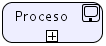
\includegraphics[width=71pt]{images/procesos/SubProceso}}%
 	\caption{Representación de un Proceso y/o Subproceso.}
 	\label{Intro:iProceso}
 	\end{figure}
% 	\begin{figure}[!h]
% 	\centering\noindent{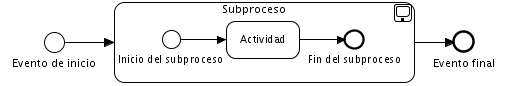
\includegraphics[width=360pt]{images/procesos/bpmn/ExpandedSubprocess.png}}%
% 	\caption{Diagrama de un subproceso expandido.}
% 	\label{Intro:ExpandedSubprocess}
% 	\end{figure}

{\bf Tarea o Actividad.} Es el grado de especificación más simple de un proceso (i.e; es el máximo detalle al que puede llegar un proceso) y de ella no pueden derivar más subprocesos o tareas. Está representado por la Figura \ref{Intro:iTarea}.
 	\begin{figure}[!h]
 	\centering\noindent{
\includegraphics[width=68pt]{images/procesos/Tarea}}%
 	\caption{Representación de una Tarea.}
 	\label{Intro:iTarea}
 	\end{figure}
% 	\begin{figure}[!h]
% 	\centering\noindent{
\includegraphics[width=240pt]{images/procesos/bpmn/SubprocessDiagram.png}}%
% 	\caption{Diagrama de un subproceso colapsado.}
% 	\label{Intro:CollapsedSubprocess}
% 	\end{figure}


%---------------------------------------------------------
\subsection{Subprocesos expandidos y contraídos}

{\bf Subproceso expandido.} Los subprocesos en BPMN, pueden representarse como se muestra en la Figura \ref{Intro:ExpandedSubprocess}. Esto significa que un subproceso puede contener varias actividades o subprocesos ``hijos''.
	\begin{figure}[!h]
	\centering\noindent{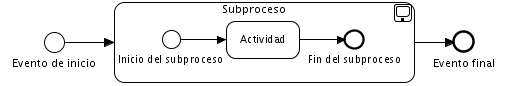
\includegraphics[width=360pt]{images/procesos/bpmn/ExpandedSubprocess.png}}%
	\caption{Subproceso expandido.}
	\label{Intro:ExpandedSubprocess}
	\end{figure}

{\bf Subproceso contraído.} Los subprocesos en BPMN, también pueden representarse como se muestra en la Figura \ref{Intro:CollapsedSubprocess}. Esta representación significa lo mismo que la Figura \ref{Intro:ExpandedSubprocess}, pero sin mostrar explícitamente sus actividades o subprocesos ``hijos''.
	\begin{figure}[!h]
	\centering\noindent{
\includegraphics[width=260pt]{images/procesos/bpmn/CollapsedSubprocess.png}}%
	\caption{Subproceso contraído.}
	\label{Intro:CollapsedSubprocess}
	\end{figure}

% {\bf Diagrama de un subproceso.} Los subprocesos en BPMN, también pueden representarse como en la Figura \ref{Intro:ExpandedCollapsed}. Esta representación significa lo mismo que la Figura \ref{Intro:ExpandedSubprocess}, pero sin mostrar explícitamente sus actividades o subprocesos ``hijos''.
% 	\begin{figure}[!h]
% 	\centering\noindent{
\includegraphics[width=360pt]{images/procesos/bpmn/SubprocessDiagram.png}}%
% 	\caption{Intro:Activity}
% 	\label{Intro:CollapsedSubprocess}
% 	\end{figure}


%---------------------------------------------------------
\subsection{Eventos}

Un {\bf evento} en BPMN representa algo que sucede o podría suceder durante el curso de un proceso y que afecta su flujo. Existen diferentes tipos de eventos:

\begin{itemize}
	\item {\bf Eventos iniciales}. Estos eventos inician el flujo del proceso y no tienen flujos de entrada.

	\arrayrulecolor{white}%
	\begin{tabular}{| m{.08\textwidth} m{.77\textwidth} | }% %{| c{.08\textwidth}  c{.77\textwidth} | }%
		\rowcolor[gray]{0.97}%
		\centering\noindent
\includegraphics[width=18pt]{images/procesos/bpmn/StartEvent.png} & {\bf Evento inicial simple}. No se especifica algún comportamiento en particular para empezar un proceso. \\
		\centering\noindent
\includegraphics[width=18pt]{images/procesos/bpmn/MessageEventStart.png} & {\bf Evento inicial de mensaje}. Un proceso empieza cuando un mensaje es recibido. \\
		\rowcolor[gray]{0.97}%
		\centering\noindent
\includegraphics[width=18pt]{images/procesos/bpmn/TimerEventStart.png} & {\bf Evento inicial de tiempo}. Un proceso empieza en determinada fecha o tiempo específico.
	\end{tabular}%

	\item {\bf Eventos intermedios}. Indican que algo ocurre o podría ocurrir en alguna parte del proceso (desde el inicio y hasta el final). Estos eventos pueden ser usados como parte del flujo de secuencia o adjuntarse a los bordes de una actividad para indicar que la actividad se ejecuta una vez que el evento es activado.

	\arrayrulecolor{white}%
	\begin{tabular}{| m{.08\textwidth} m{.77\textwidth} | }%
		\rowcolor[gray]{0.97}%
		\centering\noindent
\includegraphics[width=18pt]{images/procesos/bpmn/MessageEvent.png} & {\bf Evento intermedio de mensaje}. Indica que un mesaje puede ser enviado o recibido en alguna parte del proceso. \\
		\centering\noindent
\includegraphics[width=18pt]{images/procesos/bpmn/TimerEventIntermediate.png} & {\bf Evento intermedio de tiempo}. Indica que el proceso debe esperar un tiempo especifico para poder continuar.\\
		\rowcolor[gray]{0.97}%
		\centering\noindent
\includegraphics[width=18pt]{images/procesos/bpmn/ConditionalIntermediateEvent.png} & {\bf Evento intermedio de condición}. Se usa cuando el flujo necesita esperar por una condición de negocio para ser completado. Sólo puede usarse dentro de la secuencia del flujo o adjuntado a los bordes de una actividad para indicar que existe un flujo de excepción. \\
		\centering\noindent
\includegraphics[width=18pt]{images/procesos/bpmn/MultipleIntermediateEvent.png} & {\bf Evento intermedio múltiple}. Este evento puede ser activado por muchas causas o sólo por una de ellas. Sólo puede usarse dentro de la secuencia del flujo.\\
		\rowcolor[gray]{0.97}%
		\centering\noindent
\includegraphics[width=18pt]{images/procesos/bpmn/LinkIntermediateEvent.png} & {\bf Evento intermedio de condición}. Este evento permite conectar dos secciones del proceso y puede ser usado únicamente dentro del flujo del proceso.\\
		\centering\noindent
\includegraphics[width=18pt]{images/procesos/bpmn/CompensationIntermediateEvent.png} & {\bf Evento intermedio de compensación}. Permite manejar compensaciones. Puede ser usado dentro de la secuencia del flujo para indicar que se requiere una compensación, o adjuntado a los bordes de una actividad para indicar que la actividad será compensada una vez que el evento sea activado.
	\end{tabular}%

	\item {\bf Eventos finales}. Estos eventos finalizan el flujo del proceso, por lo tanto no pueden tener flujos de salida.

	\arrayrulecolor{white}%
	\begin{tabular}{| m{.08\textwidth} m{.77\textwidth} | }%
		\rowcolor[gray]{0.97}%
		\centering\noindent
\includegraphics[width=18pt]{images/procesos/bpmn/EndEvent.png} & {\bf Evento final.} Indica que el proceso y todas las actividades terminan, sin importar que alguna haya quedado pendiente. \\
		\centering\noindent
\includegraphics[width=18pt]{images/procesos/bpmn/LinkEvent.png} & {\bf Evento final de liga}. Este evento permite conectar dos secciones del proceso. Sólo puede usarse dentro del flujo del proceso.\\
		\centering\noindent
\includegraphics[width=18pt]{images/procesos/bpmn/CancelEndEvent.png} & {\bf Evento final de cancelación}. Permite enviar una excepción de error cuando el flujo llega al final. Este evento solo puede usarse en subprocesos.
	\end{tabular}%
\end{itemize}

%---------------------------------------------------------
\subsection{Compuertas}

Las {\bf compuertas} son elementos usados para controlar la divergencia y convergencia del flujo (separar y unir).\\

	\arrayrulecolor{white}%
	\begin{tabular}{| m{.08\textwidth} m{.77\textwidth} | }%
		\rowcolor[gray]{0.97}%
		\centering\noindent
\includegraphics[width=25pt]{images/procesos/bpmn/ExclusiveGateway.png} & {\bf Compuerta exclusiva basado en los datos}. Como decisión exclusiva, tiene dos o más flujos de secuencia alternos, pero solo uno de ellos puede tomarse basado en la condición de los datos. Como convergencia, es usado para mezclar rutas alternas en una sola. \\
		\centering\noindent
\includegraphics[width=25pt]{images/procesos/bpmn/ParallelGateway.png} & {\bf Compuerta paralela}. Como divergencia, es usada para crear rutas paralelas. Como convergencia, sincroniza multiples rutas paralelas en una. El flujo continúa cuando todas las rutas alcanzan la compuerta. \\
		\rowcolor[gray]{0.97}%
		\centering\noindent
\includegraphics[width=25pt]{images/procesos/bpmn/InclusiveGateway.png} & {\bf Compuerta inclusiva}. Como divergencia, es usada cuando en un punto del flujo una o más rutas puden ser activadas y la decisión está basada en los datos del proceso. Como convergencia, indica que las rutas activas son sincronizadas en una sola.
	\end{tabular}%

%---------------------------------------------------------
\subsection{Conectores}

Los {\bf conectores} son elementos usados para conectar objetos (tareas, subprocesos, eventos, compuertas, etc.) dentro del flujo.\\

	\arrayrulecolor{white}%
	\begin{tabular}{| m{.33\textwidth}  m{.52\textwidth} | }%
		\rowcolor[gray]{0.97}%
		\centering\noindent
\includegraphics[width=120pt]{images/procesos/bpmn/SequenceFlow.png} & {\bf Flujo de secuencia}. Representa el control del flujo y la secuencia de las actividades, compuertas y eventos. \\
		\centering\noindent
\includegraphics[width=120pt]{images/procesos/bpmn/MessageFlow.png} & {\bf Flujo de mensaje}. Es usado para mostrar el flujo de mensajes entre dos entidades o procesos. Representa señales o mensajes, {\bf no el control del flujo}. {\bf No todos los flujos de mensaje son secuenciales o esto especificaría orden en los mensajes}.
	\end{tabular}%


%---------------------------------------------------------
\subsection{Contenedores}

Un {\bf contenedor} es un elemento utilizado en BPMN para distinguir visualmente las responsabilidades entre las áreas u organizaciones.\\

	\arrayrulecolor{white}%
	\begin{tabular}{| m{.33\textwidth}  m{.52\textwidth} | }%
		\rowcolor[gray]{0.97}%
		\centering\noindent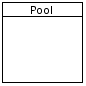
\includegraphics[width=45pt]{images/procesos/bpmn/Pool.png} & {\bf Pool}. Un {\it pool} es un contenedor representando un sólo proceso. \\%El nombre del {\it pool} puede ser considerado el nombre del proceso. \\
		\centering\noindent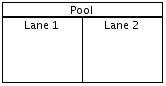
\includegraphics[width=70pt]{images/procesos/bpmn/Lane.png} & {\bf Lane}. Un {\it lane} es una subdivisión de un {\it pool} y representa un rol o área organizacional.
	\end{tabular}%

%---------------------------------------------------------
\subsection{Tipos de subprocesos}

%El {\bf proceso RENIECYT} describe una parte de la funcionalidad del registro RENIECYT, por medio de una serie de actividades bien definidas, con el objetivo de realizar el registro de los usuarios en RENIECYT.\\

Se han dividido los procesos de la \cdtRef{Actor:EscuelaLibreDeDerecho}{Escuela Libre de Derecho} en diversos subprocesos con la finalidad de entender y visualizar mejor su funcionalidad. Estos subprocesos se han clasificado en dos tipos:
\begin{itemize}
	\item Críticos. Son aquellos subprocesos complejos que pueden involucrar más de un subproceso y/o tareas y describen una parte sumamente importante del proceso propuesto para la \cdtRef{Actor:EscuelaLibreDeDerecho}{Escuela Libre de Derecho}. Están representados por la Figura \ref{Intro:iProcesoComplejo}.
	\begin{figure}[!h]
	\centering\noindent{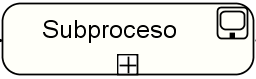
\includegraphics[width=71pt]{images/procesos/SubProcesoComplejo}}%
	\caption{Representación de un Subproceso Complejo.}
	\label{Intro:iProcesoComplejo}
	\end{figure}

	\item Simples. Son subprocesos sencillos y probablemente requieran únicamente de tareas para describir sus actividades. Están representados por la Figura \ref{Intro:iProceso}.
\end{itemize}

\noindent Notese que la única diferencia entre ambos es el color de relleno, los subprocesos críticos son de color amarillo, mientras que los subprocesos simples son de color azul.\\

%\noindent El proceso RENIECYT puede llevar a cabo diversas actividades las cuales pueden ser subprocesos o tareas. Se usa la Figura \ref{Intro:iProcesoComplejo} para indicar que una actividad es un subproceso crítico, la Figura \ref{Intro:iProceso} para indicar que una actividad es un subproceso simple y la Figura \ref{Intro:iTarea} para indicar que una actividad es una tarea.


%---------------------------------------------------------
\subsection{Nombre de los subprocesos}

\noindent Se usa la siguiente estructura para nombrar los subprocesos de Admisión de la \cdtRef{Actor:EscuelaLibreDeDerecho}{Escuela Libre de Derecho}:
	\begin{center}
		{\bf PP- + Tipo de Proceso + Número consecutivo + Nombre del subproceso}
	\end{center}

\noindent Donde:
\begin{itemize}
	\item{\bf PP-}. Significa que es un subproceso propuesto.
	\item{\bf Tipo de Proceso}. Puede tomar uno de los siguientes valores:
		\begin{itemize}
			\item{\bf A}. Significa que es un subproceso de Admisión.
		\end{itemize}
	\item{\bf Número consecutivo}. Estará dado por el nivel de profundidad que presente dicho subproceso. Por ejemplo, en la Figura \ref{Intro:JerarquiaProcesos} el Proceso General tiene un subproceso 1 y un subproceso 2.
		\begin{figure}[!h]
		\centering\noindent{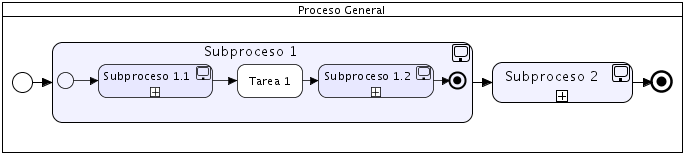
\includegraphics[width=0.87\textwidth]{images/procesos/JerarquiaProcesos_1}}%
		\caption{Subproceso General.}
		\label{Intro:JerarquiaProcesos}
		\end{figure}

		Se puede ver que el subproceso 1 tiene un subproceso 1.1, una tarea 1 y un subproceso 1.2. Si profundizáramos aún más dentro del subproceso 1.1 se verá que realiza dos actividades: tarea 1 y tarea 2, como se muestra en la Figura \ref{Intro:JerarquiaProcesos2}
		\begin{figure}[!h]
		\centering\noindent{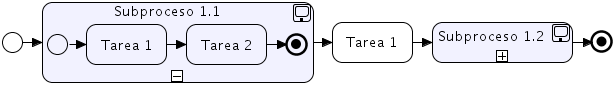
\includegraphics[width=0.8\textwidth]{images/procesos/JerarquiaProcesos2_1}}%
		\caption{Subproceso 1.1.}
		\label{Intro:JerarquiaProcesos2}
		\end{figure}

	\item{\bf Nombre del proceso}. Estará dado por el nombre que presente el subproceso o actividad en el diagrama BPMN.
\end{itemize}

\noindent Por ejemplo:
	\begin{center}
		{\bf PP-A 1.5.1 Pago SPEI}
	\end{center}

\noindent Significa que es el subproceso \textbf{PP-} de Admisión \textbf{A} número \textbf{5} que contiene el subroceso \textbf{1} llamado \textbf{Pago SPEI}.

%---------------------------------------------------------
\subsection{Elementos de un subproceso}

Un {\bf elemento} del subproceso es un atributo utilizado para describir las características de los subprocesos. Los atributos ayudan a entender la funcionalidad e interacción de un subproceso con otro (a través de los insumos de entrada y productos de salida).\\

\noindent Los elementos que describen los subprocesos de Admisión son los siguientes:

\begin{itemize}
	\item {\bf Actores:} Lista de los actores que intervienen en el subproceso.
	\item {\bf Objetivo:} Breve descripción del propósito del subproceso.
	\item {\bf Insumos de entrada:} Lista de datos de entrada requeridos durante la ejecución del subproceso.
	\item {\bf Proveedores:} Son las áreas o personas que proveen insumos al subproceso.
	\item {\bf Productos de salida:} Lista de datos de salida que otorga el subproceso al ser ejecutado.
	\item {\bf Cliente:} Áreas o personas que consumen los productos generados por el subproceso.
	\item {\bf Recursos del proceso}: Son los recursos necesarios para llevar a cabo el subproceso.
	\item {\bf Interrelación con otros procesos:} Es la interacción con otros subprocesos internos y/o externos para verificar la apropiada interacción con estos.
\end{itemize}
 % Introducción al contenido del documento

    %---------- Proceso de Admisión

	%======================EJEMPLO===================================
	\chapter{Procesos}    
    %========================================================
%Proceso
%========================================================

%========================================================
% Descripción general del proceso
%-----------------------------------------------
\begin{Proceso}{P0.1}{Solicitud de cuenta} {
  
  %-------------------------------------------
  %Resumen

  Proceso que realiza el \cdtRef{Actor:Aspirante}{Aspirante} como primer paso para obtener una cuenta activa de usuario en el \cdtRef{Actor:SAEV2.0}{SAEV2.0}, y así poder iniciar el proceso de admisión a alguna de las opciones de posgrado que la escuela ofrece.
  
  Si el periodo de registro se encuentra vigente, el sistema permite al \cdtRef{Actor:Aspirante}{Aspirante} ingresar la información necesaria para obtener el correo de activación de su cuenta, de lo contrario le notifica que se encuentra fuera de dicho periodo y por lo tanto no se puede generar su cuenta en el sistema. Cuando procede la solicitud de cuenta, el sistema verifica ahora si la información proporocionada es correcta, de no ser el caso, se notifica que existen errores en la información para que se realicen las correcciones pertinentes antes de su envío.

  Una vez que la información es enviada correctamente, el \cdtRef{Actor:SAEV2.0}{SAEV2.0} debe asegurarse de que el \cdtRef{Actor:Aspirante}{Aspirante} no se encuentra previamente registrado como \cdtRef{Actor:Aspirante}{Aspirante} con cuanta activa o como \cdtRef{Actor:Alumno}{Alumno} activo o en baja (ya sea académica, voluntario o definitiva), pues de darse alguno de estos casos, el sistema notifica que la solicitud de cuenta no procede, explicando los motivos. Si no se da alguno de los casos anteriores, el sistema termina el proceso de solicitud de cuenta realizando el envío de un correco electrónico que permitirá la activación de la cuenta de usuario generada.

  %-------------------------------------------
  %Diagrama del proceso

  \noindent La Figura \cdtRefImg{P0.1}{Solicitud de cuenta} muestra las actividades que se realizan para llevar a cabo el proceso descrito anteriormente.

  \Pfig[0.95]{./procesos/Ejemplo/Images/PA2_1-SolicitudDeCuenta.png}{P0.1}{Solicitud de cuenta}

} {P0.1:Cuenta}

  %-------------------------------------------
  %Elementos del proceso

  \UCitem{Actores} { %Actores
    \cdtRef{Actor:Aspirante}{Aspirante} y \cdtRef{Actor:SAEV2.0}{SAEV2.0}.
  }

  \UCitem{Objetivo} { %Objetivo
    Generar una cuenta de usuario sin activar y el correo de activación de la misma.
  }

  \UCitem{Insumos de entrada} { %Insumos de entrada
  	\begin{UClist}
  		\UCli Datos del formulario \cdtIdRef{F1}{Generación de cuenta}
     	\UCli  \cdtIdRef{D0.1}{Credencial de Estudiante}.
    \end {UClist}
  }
  
  \UCitem{Proveedores} { %Proveedores
    \cdtRef{Actor:Aspirante}{Aspirante}
  }

  \UCitem{Productos de salida} { %Productos de salida
    \begin{UClist}
      \UCli Notificación \cdtIdRef{MSJ0.1}{Solicitud fuera de periodo de registro}.
      \UCli Notificación \cdtIdRef{MSJ0.2}{Operacion Exitosa}.
    \end{UClist}
  }

  \UCitem{Cliente} { %Cliente
    \cdtRef{Actor:Aspirante}{Aspirante}
  }

  \UCitem{Mecanismo de medición} { %Mecanismo de medición
    \begin{UClist}
      \UCli Un día hábil  de asignación
      \UCli Cuatro días  hábiles de evaluación
    \end{UClist}
  }
  \UCitem{Interrelación con otros procesos} { %Interrelación con otros procesos
    \cdtIdRef{P0.1}{Solicitud de cuenta}
  }


\end{Proceso}

%========================================================
%Descripción de tareas
%-----------------------------------------------
\begin{PDescripcion}

  %Actor: Aspirante
  \Ppaso Aspirante

    \begin{enumerate}

      %Tarea a
      \Ppaso[\itarea] \cdtLabelTask{T1-P0.1:Aspirante}{Solicita cuenta de usuario.} Para obtener una cuenta de usuario en el \cdtRef{Actor:SAEV2.0}{SAEV2.0}, ésta debe solicitarse durante el periodo de registro de aspirantes mostrando la \cdtIdRef{D0.1}{Credencial de Estudiante}. Una vez realizada la solicitud, se espera a que suceda uno de los siguientes eventos:

	%Eventos
	\begin{itemize}
	  %Evento 1
	  \item Se autoriza la generación de cuenta. Si el \cdtRef{Actor:SAEV2.0}{SAEV2.0} determina que la solicitud esta dentro del periodo de registro, autoriza la generación de la cuenta y se puede pasar a la tarea \cdtRefTask{T2-P0.1:Aspirante}{Ingresa información}, para iniciar la creación de la cuenta en el sistema.
	  %Evento 2
	  \item Recibe notificación de solicitud fuera de periodo. Si el \cdtRef{Actor:SAEV2.0}{SAEV2.0} determina que la solicitud esta fuera del periodo de registro, se recibe la notificación \cdtIdRef{MSJ0.1}{Solicitud fuera de periodo de registro}, la cual indica que no puede proceder la solicitud.
	\end{itemize}

      %Tarea b
      \Ppaso[\itarea] \cdtLabelTask{T2-P0.1:Aspirante}{Ingresa información.} Proporciona los datos  especificados en el formulario \cdtIdRef{F1}{Generación de cuenta}, y una vez que envía la información al \cdtRef{Actor:SAEV2.0}{SAEV2.0}, queda a la espera de que suceda alguno de los siguientes eventos:

	%Eventos
	\begin{itemize}
	  %Evento 1
	  \item Recibe notificación de error en la información. Indica que la información proporcionada al sistema no puede ser registrada, y los detalles se especifican en la notificación \cdtIdRef{NS2}{Información errónea} enviada por el \cdtRef{Actor:SAEV2.0}{SAEV2.0}. Para realizar los ajustes correspondientes, pasa a la tarea \cdtRefTask{T2-P0.1:Aspirante}{Ingresa información}.
	  %Evento 2
	  \item Recibe notificación de cuenta denegada por baja. Indica que la solicitud de cuenta es denegada, debido a que la información ingresada corresponde a un \cdtRef{Actor:Alumno}{Alumno} dado de baja ya sea académica, voluntaria o definitiva, y el proceso termina. Lo anterior se especifica en la notificación \cdtIdRef{NS3}{Cuenta denegada por baja}, enviada por el \cdtRef{Actor:SAEV2.0}{SAEV2.0}.
	  %Evento 3
	  \item Recibe notificación de cuenta con activación inhabilitada. Indica que ya se tiene una cuenta registrada y que su activación ha sido inhabilitada, por lo que es necesario que pase al proceso \cdtIdRef{P0.1}{Activación de cuenta} para poder activarla, y el proceso termina. Lo anterior se detalla en la notificación \cdtIdRef{NS4}{Cuenta con activación inhabilitada} enviada por el \cdtRef{Actor:SAEV2.0}{SAEV2.0}.
	  %Evento 4
	  \item Recibe notificación de cuenta por activar. Indica que ya se tiene una cuenta registrada y que necesita ser activada, por lo que es necesario que pase al proceso \cdtIdRef{P0.1}{Activación de cuenta} para poder activarla, y el proceso termina. Lo anterior se detalla en la notificación \cdtIdRef{NS5}{Cuenta por activar} enviada por el \cdtRef{Actor:SAEV2.0}{SAEV2.0}.
	  %Evento 5
	  \item Recibe notificación de cuenta previa existente. Indica que ya se tiene una cuenta activa en el sistema ya sea como \cdtRef{Actor:Aspirante}{Aspirante} o como \cdtRef{Actor:Alumno}{Alumno}, por lo que la solicitud de cuenta no procede y el proceso termina. Lo anterior se detalla en la notificación \cdtIdRef{NS6}{Cuenta previa activada} enviada por el \cdtRef{Actor:SAEV2.0}{SAEV2.0}.
	  %Evento 6
	  \item Recibe notificación de solicitud de activación de cuenta. Indica que el sistema ha creado la cuenta, la cual necesita ser activada para poder ser utilizada. Para realizar dicha activación, se recibe vía correo electrónico la notificación \cdtIdRef{NS7}{Activación de cuenta} por parte del \cdtRef{Actor:SAEV2.0}{SAEV2.0}. El proceso termina exitósamente y se puede activar la cuenta en el proceso \cdtIdRef{P0.1}{Activación de cuenta}.
	\end{itemize}

    \end{enumerate}

  %Actor: SAEV2.0
  \Ppaso SAEV2.0

    \begin{enumerate}

      %Tarea a
      \Ppaso[\itarea] \cdtLabelTask{T1-P0.1:SAEV2.0}{Autoriza la creación de cuenta.} Para que el sistema autorice una solicitud de creación de cuenta de usuario, éste debe verificar la condición \cdtIdRef{C1}{Solicitud fuera de periodo de registro}. Si la condición es falsa, es decir, la solicitud esta dentro del periodo de registro, el sistema pasa a la tarea \cdtRefTask{T3-P0.1:SAEV2.0}{Genera cuenta.} Cuando la condición es verdadera, es decir, la solicitud esta fuera del periodo de registro, el sistema pasa a la tarea \cdtRefTask{T2-P0.1:SAEV2.0}{Notifica solicitud fuera de periodo de registro.}

      %Tarea b
      \Ppaso[\itarea] \cdtLabelTask{T2-P0.1:SAEV2.0}{Notifica solicitud fuera de periodo de registro.} Muestra la notificación \cdtIdRef{NS1}{Solicitud fuera de periodo de registro}, donde indica que no se puede crear la cuenta de usuario por estar fuera de dicho periodo, por lo que no puede continuar el proceso.

      %Tarea c
      \Ppaso[\itarea] \cdtLabelTask{T3-P0.1:SAEV2.0}{Genera cuenta.} Una vez que se ha autorizado la creación de la cuenta, antes de registrar la información enviada por el \cdtRef{Actor:Aspirante}{Aspirante} mediente el formulario \cdtIdRef{F1}{Generación de cuenta}, el sistema verifica que no haya errores en la información. Si se presenta algun error al procesar la información, el sistema pasa a la tarea \cdtRefTask{T4-P0.1:SAEV2.0}{Notifica error en la información.} Si la información es correcta, el sistema verifica ahora que no se cumpla alguna de las siguientes condiciones:

	%Condiciones
	\begin{itemize}
	  %Condición
	  \item \cdtIdRef{C0.1}{Alumno en baja.} el sistema pasa a la tarea \cdtRefTask{T5-P0.1:SAEV2.0}{Notifica rechazo por baja.}
	  %Condición
	  \item \cdtIdRef{C0.3}{Cuenta con activación inhabilitada.} el sistema pasa a la tarea \cdtRefTask{T6-P0.1:SAEV2.0}{Notifica cuenta con activación inhabilitada.} 
	  %Condición
	  \item \cdtIdRef{C0.4}{Cuenta por activar.} el sistema pasa a la tarea  \cdtRefTask{T7-P0.1:SAEV2.0}{Notifica cuenta por activar.}
	  %Condición
	  \item \cdtIdRef{C0.5}{Cuenta previa activada.} el sistema pasa a la tarea \cdtRefTask{T8-P0.1:SAEV2.0}{Notifica cuenta previa activada.}
	\end{itemize}

      Si no se cumple alguna de las condiciones anteriores, el sistema registra la información, crea la cuenta del usuario y el sistema pasa a la tarea \cdtLabelTask{T9-P0.1:SAEV2.0}{Notifica solicitid de activación de cuenta.}.

      %Tarea d
      \Ppaso[\itarea] \cdtLabelTask{T4-P0.1:SAEV2.0}{Notifica error en la información.} Muestra la notificación \cdtIdRef{NS2}{Información errónea en formulario}, donde indica que no se pueden procesar los datos recibidos debido a que no son correctos, y pasa a la tarea \cdtRefTask{T3-P0.1:SAEV2.0}{Genera cuenta.}, para recibir nuevamente la información.

      %Tarea e
      \Ppaso[\itarea] \cdtLabelTask{T5-P0.1:SAEV2.0}{Notifica rechazo por baja.} el sistema envía la notificación \cdtIdRef{NS3}{Cuenta denegada por baja}

      %Tarea f
      \Ppaso[\itarea] \cdtLabelTask{T6-P0.1:SAEV2.0}{Notifica cuenta con activación inhabilitada.} el sistema envía la notificación \cdtIdRef{NS4}{Cuenta con activación inhabilitada}

      %Tarea g
      \Ppaso[\itarea] \cdtLabelTask{T7-P0.1:SAEV2.0}{Notifica cuenta por activar.} el sistema envía la notificación \cdtIdRef{NS5}{Cuenta por activar}

      %Tarea h
      \Ppaso[\itarea] \cdtLabelTask{T8-P0.1:SAEV2.0}{Notifica cuenta previa activada.} el sistema envía la notificación \cdtIdRef{NS6}{Cuenta activada previamente}

      %Tarea i
      \Ppaso[\itarea] \cdtLabelTask{T9-P0.1:SAEV2.0}{Notifica solicitid de activación de cuenta.} el sistema envía la notificación \cdtIdRef{MSJ0.2}{Operacion Exitosa}

    \end{enumerate}

\end{PDescripcion}
 		%PA2.1 Generación de cuenta 

%====================CELULA1=====================================
%Introducir los correspondientes a la GESTIÓN DE EMPLEADOS



%====================CELULA2=====================================
%Introducir los correspondientes a la GESTIÓN DE INVENTARIO



%====================CELULA3=====================================
%Introducir los correspondientes a la GESTIÓN DE PRÉSTAMOS



%====================CELULA4=====================================
%Introducir los correspondientes a la GESTIÓN DE USUARIOS



%====================CELULA5=====================================
%Introducir los correspondientes a la GESTIÓN DE CREDENCIALES


    
    
    %---------- Actores
    %=============================================
% Descripción de actores

\chapter{Actores del sistema}
\label{chapter:ActoresDelSistema}

En el presente capítulo se definen los actores que participan en el sistema.


%==============Aspirante=========================================
\cdtLabel{Actor:Aspirante}{}
\begin{Actor}{Aspirante}{}
	\item[Área:] No aplica
	\item[Responsabilidades:] \hspace{1pt}
	\begin{itemize}
		\item Crear su cuenta de usuario para poder acceder al SAEV2.0.
		\item Llenar su solicitud  en tiempo y forma.
		\item Realizar los pagos necesarios para la realización del tramite.
		\item Presentar el examen del CENEVAL y el psicométrico.
		\item Crear su cuenta de usuario en el sistema.
		\item Realizar el registro de su solicitud de ingreso durante el periodo establecido.
		\item Realizar el pago de derechos a exámenes.
		\item Presentar los exámenes CENEVAL y psicométrico.
		\item Seleccionar un horario para la entrevista
		\item Acudir a la entrevista en la Escuela Libre de Derecho
		\item Visualizar el resultado del proceso de admisión
        \item Presentar la documentación necesaria para acreditar su persona y sus estudios.
        \item Realizar su registro de cita para entrevista en caso de ser seleccionado.
        \item Consultar el resultado del proceso de admisión a la ELD.
	\end{itemize}
	\item[Perfil:] \hspace{1pt}
	\begin{itemize}
		\item Debe ser un egresado o estar cursando el último año de nivel medio superior. 
		\item Debe ser capaz de trabajar bajo presión.
		\item Debe contar con facilidad de palabra.
		\item Debe ser responsable.		
	\end{itemize}
\end{Actor}

%==============  SAEV2.0 ========================
\cdtLabel{Actor:SAEV2.0}{}
\begin{Actor}{SAEV2.0}{Sistema de administración escolar encargado de gestionar todo lo relacionado con ----- }
	\item[Área:] ---
	\item[Responsabilidades:] \hspace{1pt}
	\begin{itemize}
		\item Generar el calendario escolar.
		\item Generar la convocatoria.
		\item Generar la cuenta de aspirante.
		\item Registrar los datos del aspirante.
		\item Registrar los folios de CENEVAL.
		\item Registrar los salones para la aplicación del examen CENEVAL.
		\item Registrar resultados de la encuesta CENEVAL.
		\item Enviar los resultados de la encuesta a CENEVAL.
		\item Procesar resultados de examen CENEVAL.
		\item Generar lista de aspirantes para entrevista y enviar notificaciones.
		\item Registrar salones, entrevistadores y horarios de disponibilidad de los entrevistadores.
		\item Registrar los datos de la entrevista.
		\item Generar lista de aspirantes aceptados en la Escuela Libre de Derecho y enviar notificaciones a los aspirantes.
	\end{itemize}
\end{Actor}
 %Actores identificados y su descripción

    %---------- Glosario
    \chapter{Glosario de términos}
\label{chapter:GlosarioDeTerminos}
    
Esta sección describe de forma breve y sencilla los términos utilizados a lo largo del documento, considerados necesarios para ayudar a comprender la jerga utilizada en los procesos de la \refActor{Escuela Libre de Derecho}.

%\section{Términos Técnicos}
%	En esta sección se definen los términos técnicos usados a lo largo de este documento:
	
\begin{description}
	\BRterm{Catálogo de Salones.} Contiene la información necesaria de los salones existentes en la \refActor{Escuela Libre de Derecho}.

	\BRterm{Examen EXANI II Admisión.}\label{glosario:EXANI II Admision} Evalúa aptitudes y competencias disciplinares predictivas del desempeño. Su propósito es detectar el potencial de los aspirantes para cursar con éxito el primer año del nivel educativo al que desean ingresar.
	\BRterm{EXANI-II Diagnóstico.}\label{glosario:EXANI II Diagnostico} Mide las competencias disciplinares esenciales que deben dominar los estudiantes para ingresar al programa de educación superior que han elegido.
	
	
\end{description}


    %---------- Anexos
    \appendix
    \cfinput{anexos/Condiciones} % Condiciones y Reglas de Negocio
    \cfinput{anexos/Mensajes} % Mensajes
    \cfinput{anexos/Formularios} % Formularios
    \cfinput{anexos/Documentos} % Documentos

    \clossing

\end{document}

